\documentclass[tikz]{standalone}

\usepackage{circuitikz}

\usetikzlibrary{positioning}

\begin{document}
	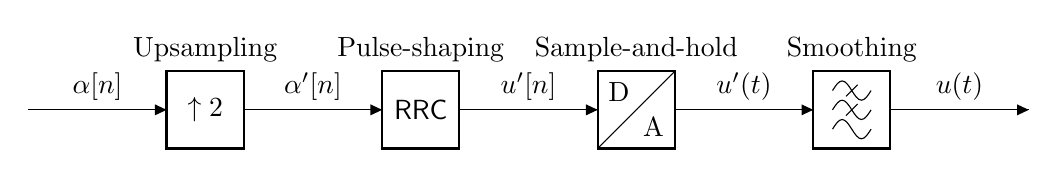
\begin{tikzpicture}[
		node distance=5em,
	]
		\coordinate (in) at (0,0);		
		\node (ups) [twoportshape, right=of in, t=$\uparrow2$] {};
		\node (psh) [twoportshape, right=of ups, t=\textsf{RRC}] {};
		\node (dac) [dacshape, right=of psh] {};
		\node (lwp) [lowpassshape, right=of dac] {};
		\coordinate[right=of lwp] (out);
		
		\draw (in) -- (ups.west) node[above, midway, sloped]{$\alpha[n]$} node[inputarrow]{};
		\draw (ups.east) -- (psh.west) node[above, midway, sloped]{$\alpha^\prime[n]$} node[inputarrow]{};
		\draw (psh.east) -- (dac.west) node[above, midway, sloped]{$u^\prime[n]$} node[inputarrow]{};
		\draw (dac.east) -- (lwp.west) node[above, midway, sloped]{$u^\prime(t)$} node[inputarrow]{};
		\draw (lwp.east) -- (out) node[above, midway, sloped]{$u(t)$} node[inputarrow]{};
		
		\node at (ups.north) [above]{Upsampling};
		\node at (psh.north) [above]{Pulse-shaping};
		\node at (dac.north) [above]{Sample-and-hold};
		\node at (lwp.north) [above]{Smoothing};
	\end{tikzpicture}
\end{document}
